%%%%%%%%%%%%%%%%%%%%%%%%%%%%%%%%%%%%%%%%%%%%%%%%%%%%
\documentclass[12pt]{article}
\usepackage{sbc-template}
\usepackage{tikz}
\usepackage{listings}
\usepackage{color}
\newcommand{\mohammad}[1]{\textcolor{red}{Mohammad: #1}}
%%%%%%%%%%%%%%%%%%%%%%%%%%%%%%%%%%%%%%%%%%%%%%%%%%%%


%%%%%%%%%%%%%%%%%%%%%%%%%%%%%%%%%%%%%%%%%%%%%%%%%%%%
\title{Abstraction Layer for Data Cleaning Tools}
\author{Milad Abbaszadeh Jahromi\inst{1}}
\address{Technische Universit\"{a}t Berlin \email{author1@tu-berlin.de}}
\begin{document} 
\maketitle
%%%%%%%%%%%%%%%%%%%%%%%%%%%%%%%%%%%%%%%%%%%%%%%%%%%%


%%%%%%%%%%%%%%%%%%%%%%%%%%%%%%%%%%%%%%%%%%%%%%%%%%%%
\begin{abstract} 
	This is the abstract...
	\mohammad{leave abstract. i will write it.}
		
	% \textbf{Keywords}: Keyword 1, Keyword 2, Keyword 3.
\end{abstract}
%%%%%%%%%%%%%%%%%%%%%%%%%%%%%%%%%%%%%%%%%%%%%%%%%%%%


%%%%%%%%%%%%%%%%%%%%%%%%%%%%%%%%%%%%%%%%%%%%%%%%%%%%
\section{Introduction}
\label{section:introduction}

\subsection{Motivation}
This report talks about the abstract layer which can help users to avoid from conflicting with the tools for cleaning purpose and help them for unique and constant input and output which can be really remarkable to save time for people who wish to work with these tools.
\mohammad{the motivation can be so much better and stronger. talk about different tools that have heterogeneity in terms of language, installation, input/output system and so on and the user difficulties.}

\subsection{Contributions}
If you have a file and wish to clean it with cleaning tools and you wouldn’t like to get involved in installation and command usage which is required for running, you can simply use our abstract layer.
With this layer you can simply send your file and then get the Suspicious element by the constant type and form in output for each tool.
\mohammad{talk about how this module can address the so-called heterogeneities for the user's application. use bullet list just like the other papers' contributions. talk about user instead of "you".}

\subsection{Architecture}
\mohammad{in this subsection talk about the big picture of the architecture and the position of the abstraction layer in the user system. I have added a proper figure. you write the texts.}
\begin{figure}[t]
	\centering
	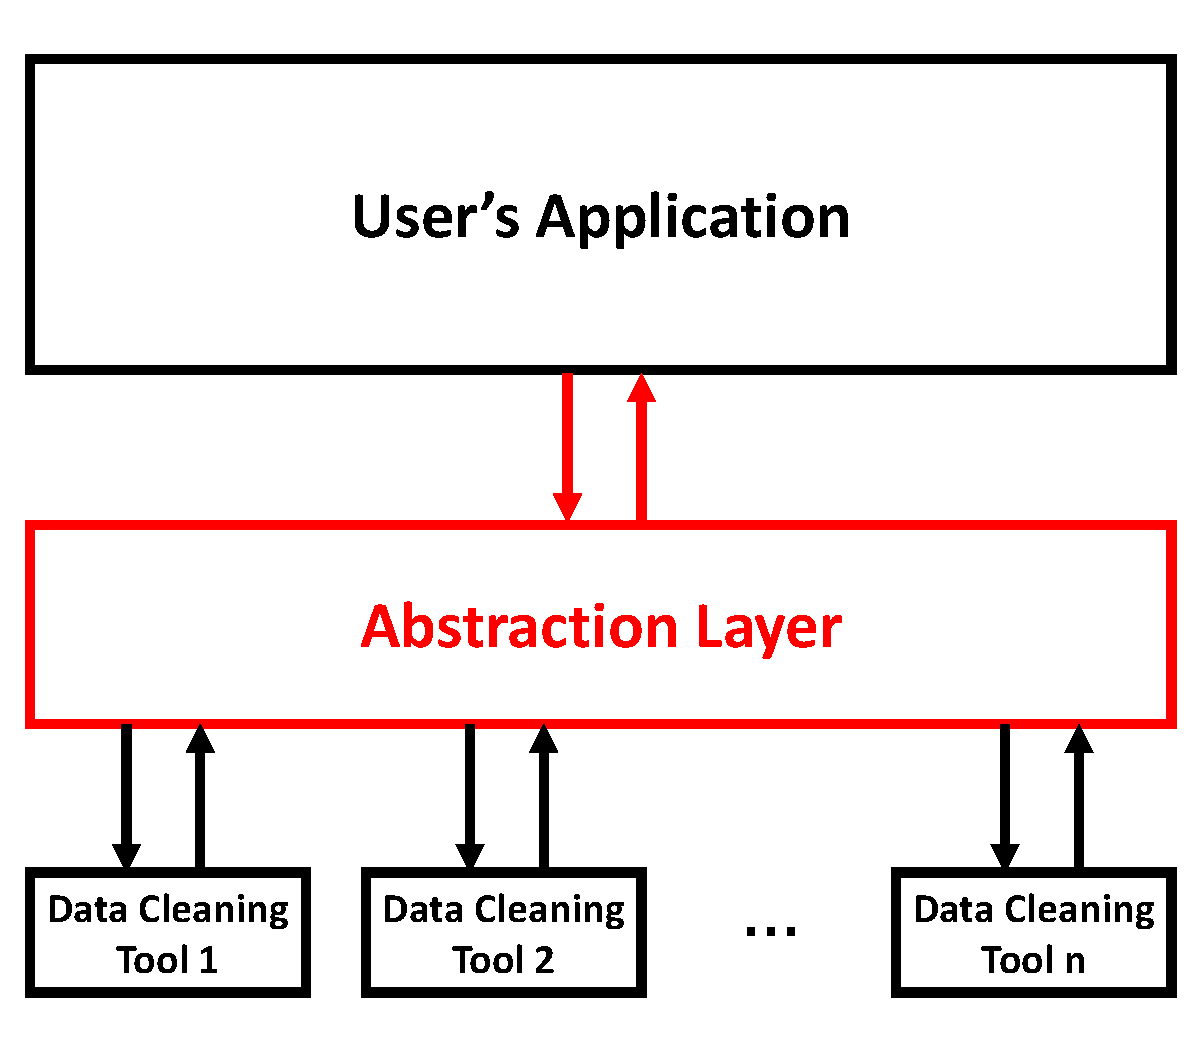
\includegraphics[scale=0.3]{attachments/architecture}
	\caption{The position of the abstraction layer in the architecture of the user's system.}
	\label{figure:architecture}
\end{figure}

\subsection{Overview}
The rest of this document is organized as follows. In Section~\ref{section:installation} we explain how the user can install the module. In Section...
\mohammad{complete this subsection}
%%%%%%%%%%%%%%%%%%%%%%%%%%%%%%%%%%%%%%%%%%%%%%%%%%%%


%%%%%%%%%%%%%%%%%%%%%%%%%%%%%%%%%%%%%%%%%%%%%%%%%%%%
\section{Installation}
\label{section:installation}

\subsection{Prerequisites}
To install the module, you need first to install followings:
\begin{itemize}
	\item Linux (Ubuntu/Debian recommended)
	\item Python 2.7
	\item Oracle Java 1.8
	\item Apache Ant 1.8.2+
	\item Postgres SQL 9.2+
\end{itemize}

\subsection{Setup}
\mohammad{talk about how the user can use the installation function in the first place to installs and configures the tools. introduce the API function that installs and configures the tools.}
%%%%%%%%%%%%%%%%%%%%%%%%%%%%%%%%%%%%%%%%%%%%%%%%%%%%


%%%%%%%%%%%%%%%%%%%%%%%%%%%%%%%%%%%%%%%%%%%%%%%%%%%%
\section{Start to Work}

\subsection{Input}
For starting with abstract layer you should make sure that you make dictionary like dictionary that is introduced below as input for our layer.
This dictionary has two keys that you can set the first one with the type of your file and the location of the file as path. In fact, for now the layer only support the files that generate with csv format but we will keep going to add other formats for future. 
\mohammad{before introducing the template of your input configuration (look below), first start to talk generally about: (1) proper api function. (2) define the argument that it needs (input configuration, data cleaning job, or whatever you call it), then you have the following codes:}
\begin{lstlisting}[language=Python]
run_input = {
	"dataset": {
		"type": "csv",
		"param": ["the/address/of/your/file.csv"]
	},
	"tool": {
		"name": "tool name",
		"param": ["list of parameters wrt. to the tool name"]
	}
}
\end{lstlisting}
\mohammad{after the general template of the input object, start to explain each key and its proper values in a nested list:}
\begin{itemize}
	\item \textbf{dataset}. This part of the input configuration is responsible to describe the input dataset. it consists of two options:
	\begin{itemize}
		\item \textbf{type}. This option specifies the type of dataset. Currently the module only supports "csv" datasets.
		\item \textbf{param}. This option specifies the list of parameters that are needed for accessing the dataset. For csv datasets, this list contains only the path of dataset.
	\end{itemize}
	\mohammad{complete this structure...}
\end{itemize}
\mohammad{after that you can provide some examples.}

\subsection{Output}
You will get one list as output that you can find it below
[row, column, suspicions value]
\mohammad{just like the input subsection, write in this subsection.}
%%%%%%%%%%%%%%%%%%%%%%%%%%%%%%%%%%%%%%%%%%%%%%%%%%%%


%%%%%%%%%%%%%%%%%%%%%%%%%%%%%%%%%%%%%%%%%%%%%%%%%%%%
\bibliographystyle{unsrt}
\bibliography{attachments/bibliography}

\end{document}
%%%%%%%%%%%%%%%%%%%%%%%%%%%%%%%%%%%%%%%%%%%%%%%%%%%%